\section{Roy Topohedron}
Isometrically compressed data from topological hypersurface to roy topohedron surface in fphase space. \newline
Prinicpal limiting nodes containing all boundary entities in a network. \newline
Surface with all i $\in$ attribute \newline
\subsection{Roy Simplex}
%1 Face of a Roy Tophedron

%\begin{figure}[H]
 % 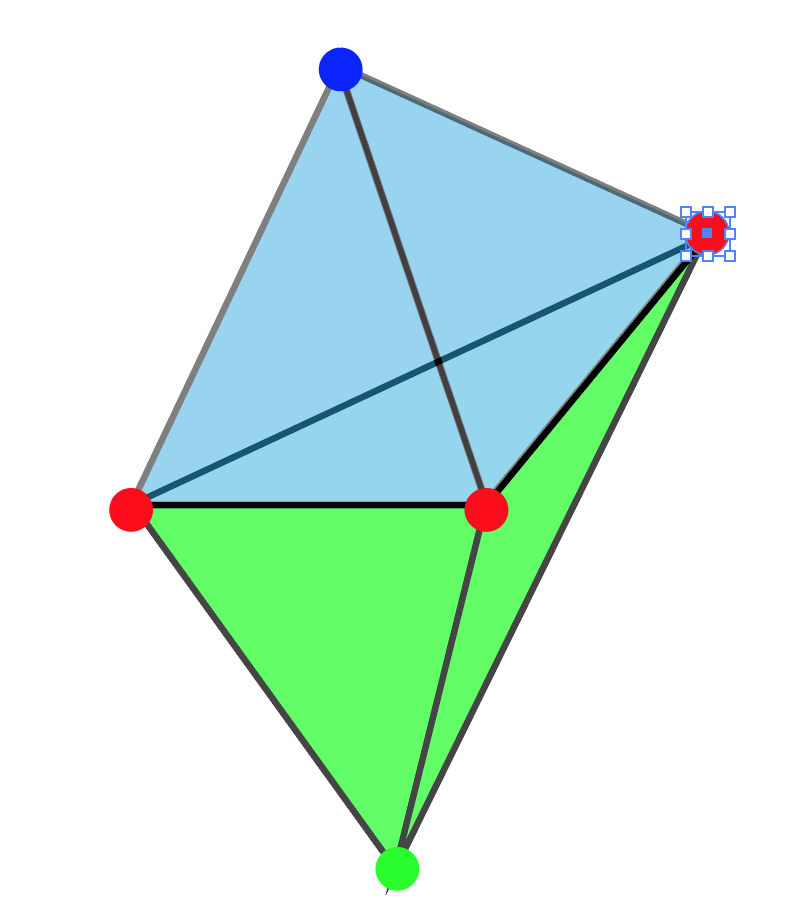
\includegraphics[width=\linewidth]{images/topohedron}
 % \caption{Roy topohedron} % Figure caption
 % \label{topohedron} 
%\end{figure}

\begin{figure}[H]
  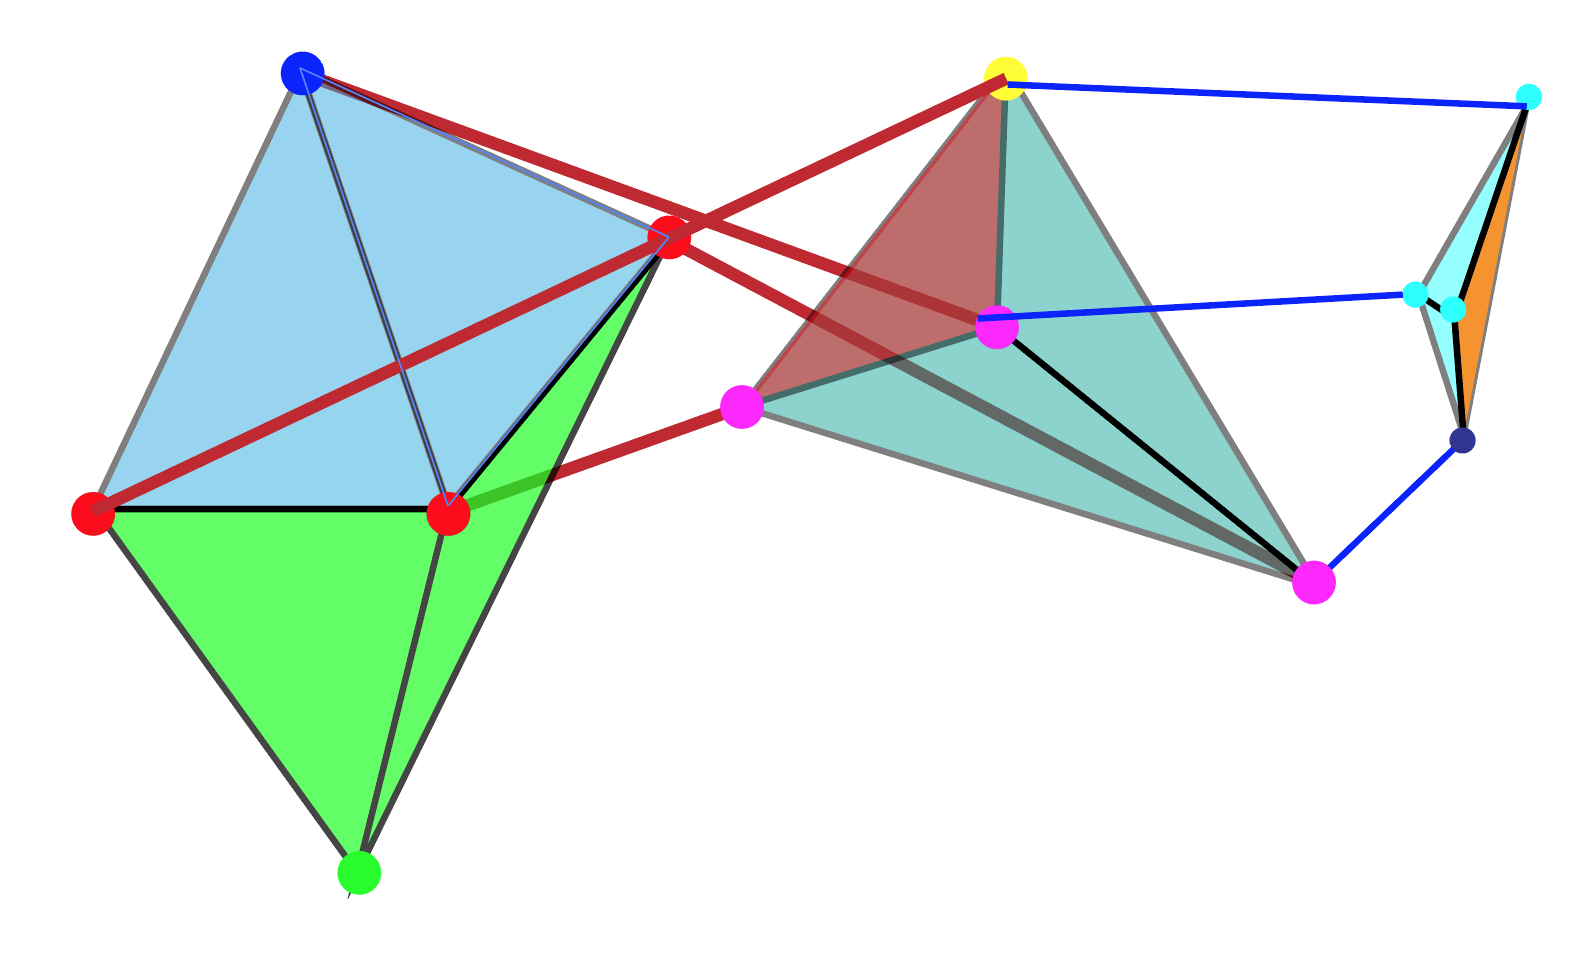
\includegraphics[width=\linewidth]{images/topoview}
  \caption{Topoview} % Figure caption
  \label{topoview} 
\end{figure}

\subsection{General Topological Properties}
Kolmogorov,Frechet,and Hausdorff space?
Seperable,
Connection properites,
Compactness Properties,
Metrizable,
Topological homogenity,
Finitely generated,
$\kappa$ resolvable
Dispersion character,
Strongly Discrete.

Simplicial Approximation Theorem
Abstract Simplical Complexes

\subsection{Topohedron Classes}


\begin{figure}[H]
  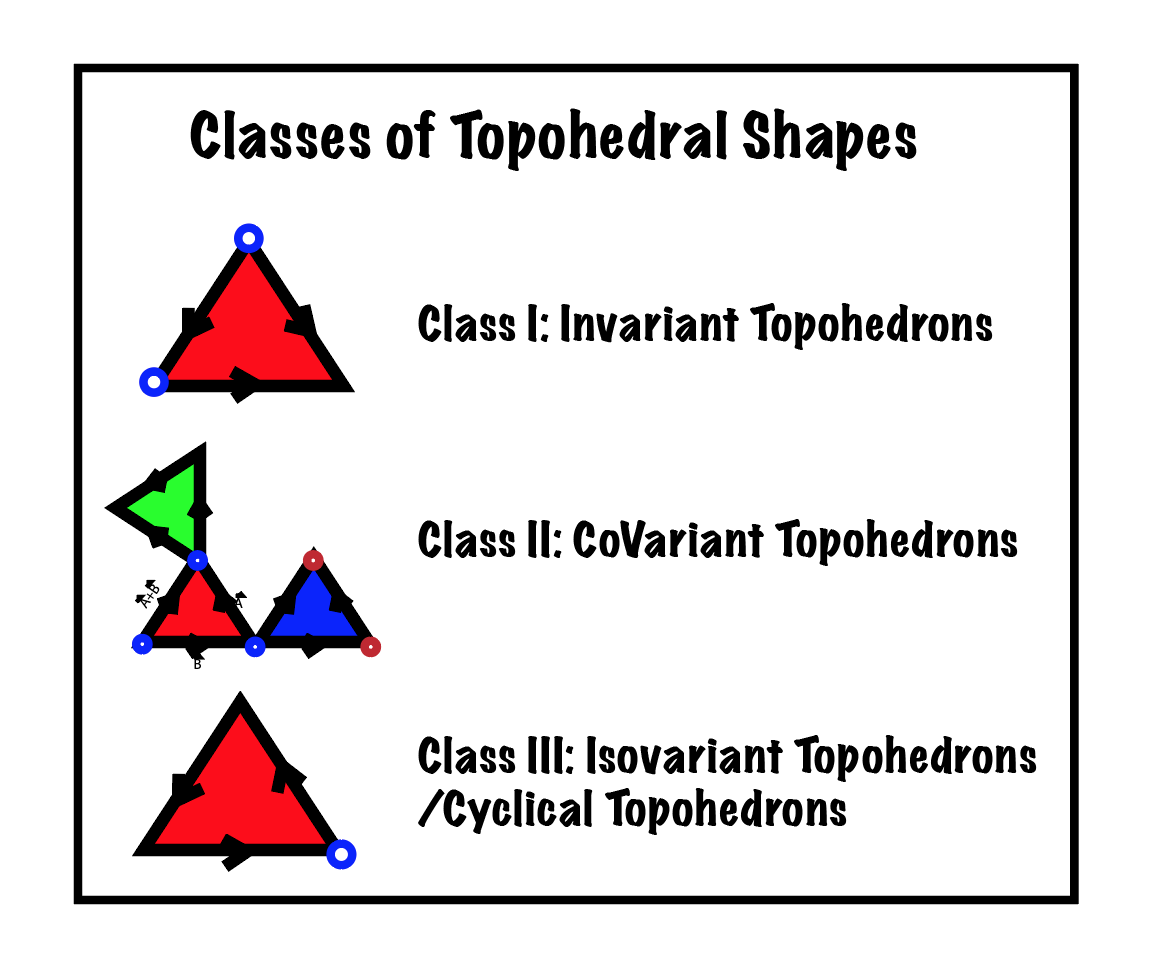
\includegraphics[width=\linewidth]{images/classes}
  \caption{Classes Explained} % Figure caption
  \label{classes} 
\end{figure}

\begin{definition}[Covariant Topohedrons]
In a covariant topohedron, at max entropy the symmetry breaks $\tau sym \in \Delta i$  \newline
Invariant under $\Delta i / \Delta S$
\end{definition}
\begin{definition}[ClassII: Invariant Topohedrons]
Invariant Topohdrons perserve symettry at $\tau sym \in \Delta i$ \newline
Covariant under $\Delta i / \Delta S$ \newline
For Both: \newline
If $\frac{W_f}{W_i} < 1 (k_i - k_f) > 0 \rightarrow class2$ \newline
If $\frac{W_f}{W_i} < 1 (k_i - k_f) < 0 \rightarrow class2$ \newline
\end{definition}


\begin{definition}[ClassIII: Isovariant Topohedrons]
Isovariant topohedrons are isolated, closed, information loops that occupy special cases of topologiacl representations.\newline
Isovariant as $\Delta i = k$
\end{definition}

\subsection{Properties}
$k_i$ is the initial size of the simplex surface\newline
$k_f$ is the final size of the simplex surface\newline
If $\frac{W_f}{W_i} \approx 1 (k_i - k_f) = 0 \rightarrow class3$\newline
If $\frac{W_f}{W_i} \ne 1 (k_i - k_f) = 0 \rightarrow class1$\newline
If $\frac{W_f}{W_i} < 1 (k_i - k_f) \ne 0 \rightarrow class2$\newline

Continutity,
Connectedness,
Convergence

\subsection{Measuring Topological Entropy}
therefore Network Entropy is defined as $\Delta S_n = \frac{\Delta K_s}{n} \times log(\frac{|W_f|}{W_i})$\newline

Check this: \footnote{https://math.uchicago.edu/~may/REU2014/REUPapers/Butt.pdf} which defined topological entropy. This also \footnote{https://www.ncbi.nlm.nih.gov/pubmed/27415290} might help, which defines the Riemannian-geometric entropy for measuring network complexity.

\subsection{Proof}
\subsection{Sample Cases}
